\documentclass[10pt,a4paper]{article}

\usepackage[utf8]{inputenc}
\usepackage[T1]{fontenc}
\usepackage{amsmath}
\usepackage{amsfonts}
\usepackage{amssymb}
\usepackage{graphicx}
\usepackage{hyperref}
\usepackage{listings}
\usepackage{xcolor}
\usepackage{float}
\usepackage[top=2cm, bottom=2cm, left=2cm, right=2cm]{geometry}
\usepackage{pgfplotstable}
\usepackage{booktabs} % for prettier tables


\title{Knowledge Graphs Project: Research Publication Domain}
\author{Jonàs Salat, Albert Vidal}

\begin{document}

\maketitle

\section{Exploring DBpedia}
[This section is for exploration purposes only, no deliverables required]

\section{Ontology Creation}
\subsection{TBOX Definition}
The TBOX (Terminological Box) defines the schema, classes, and properties of our knowledge graph. It serves as the structural foundation for our ontology.

\begin{figure}[H]
    \centering
    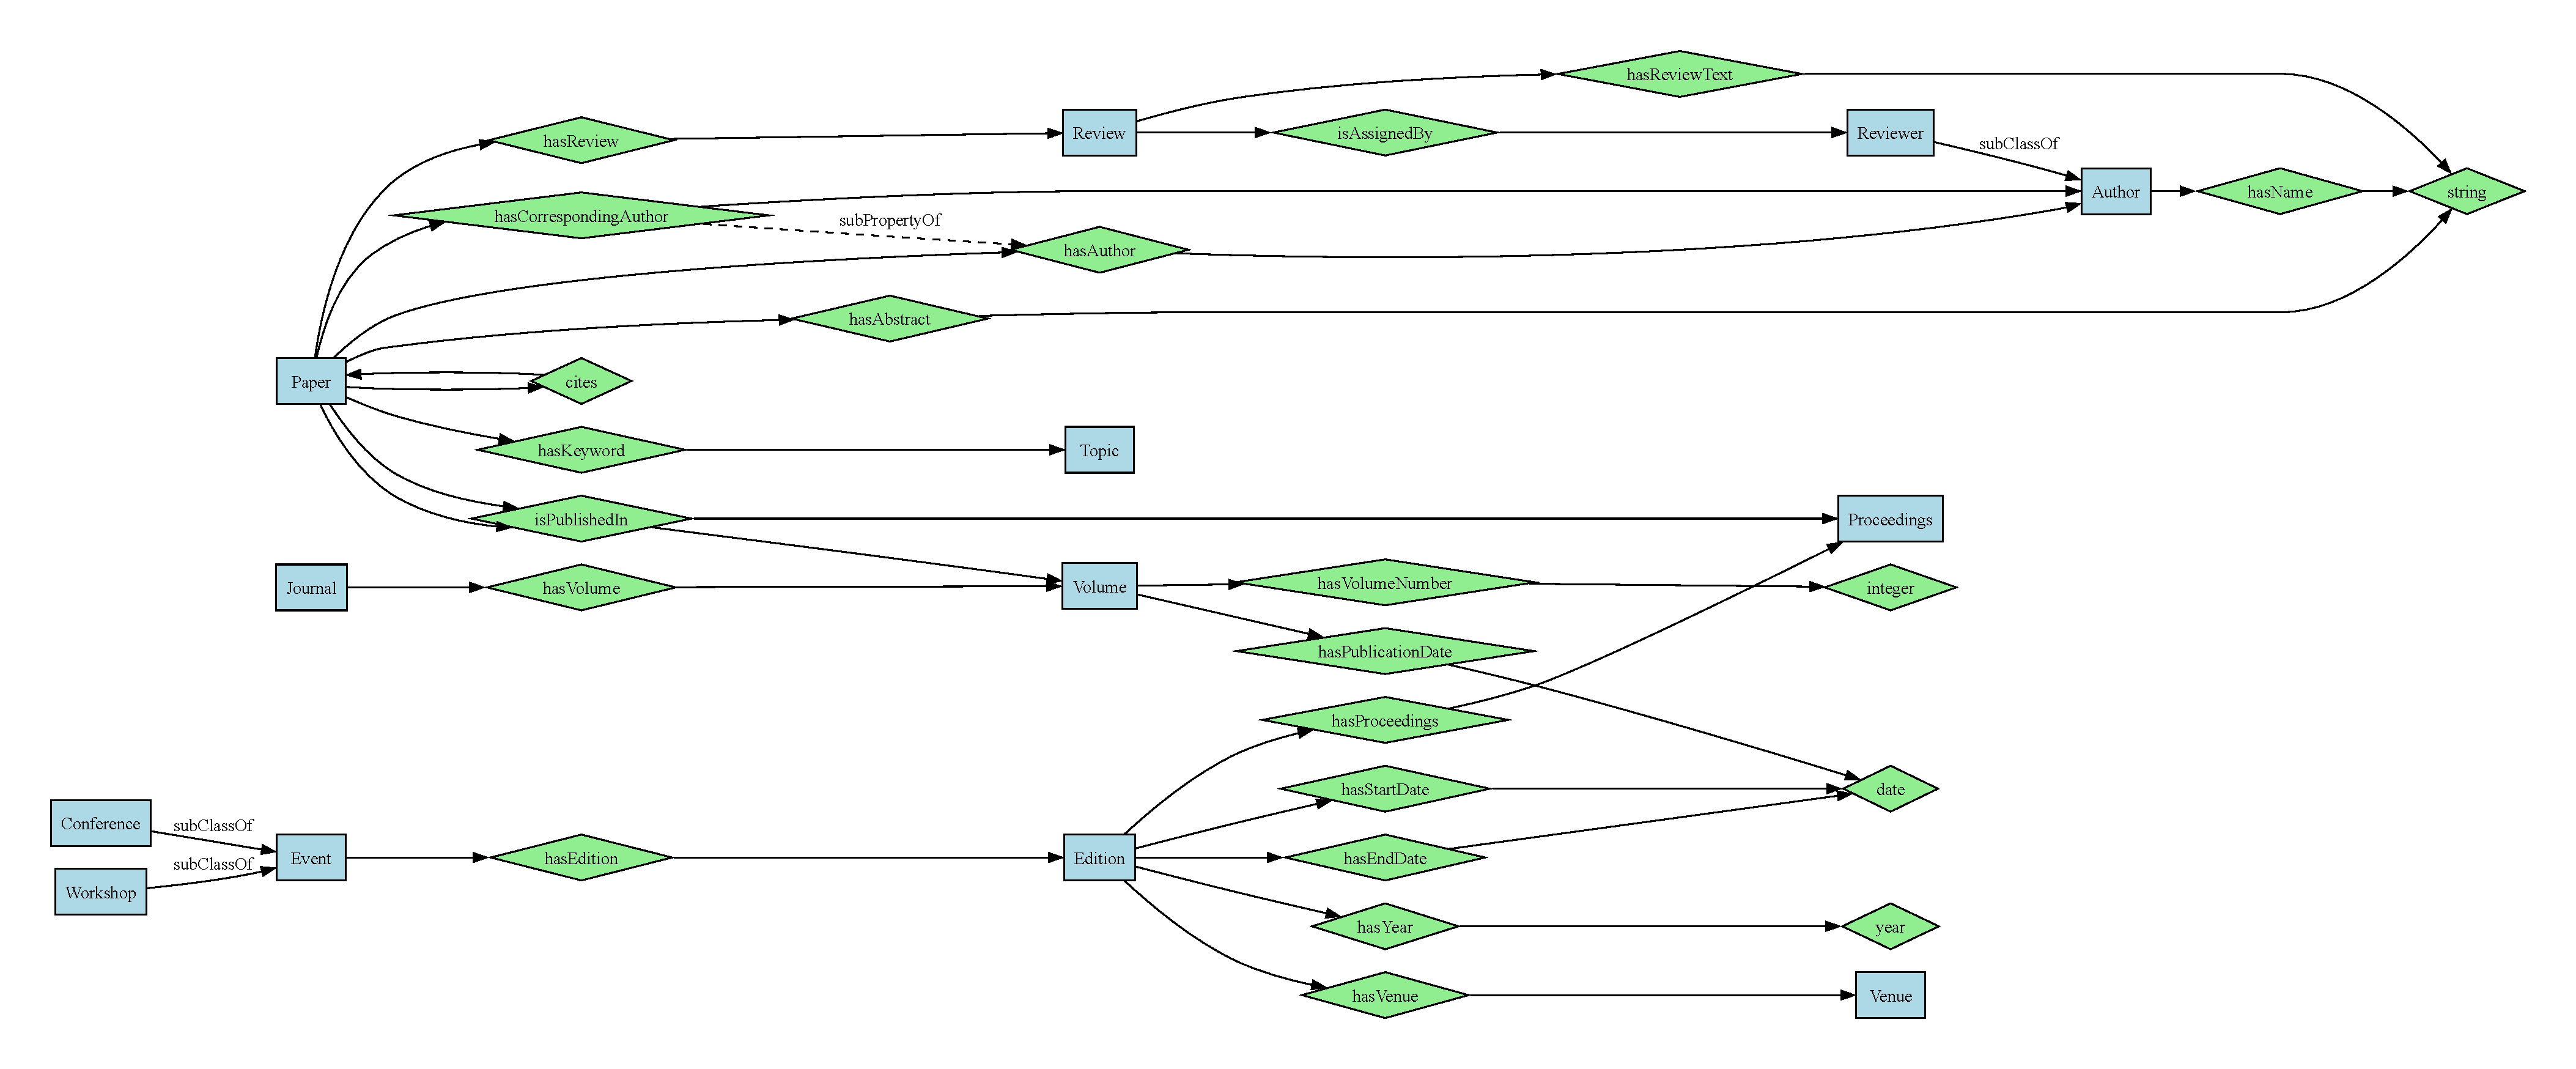
\includegraphics[width=\textwidth]{img/publication_tbox.pdf}
    \caption{Visualization of the Publication Domain TBOX showing classes, properties, and their relationships. Classes are shown in light blue boxes, properties in light green diamonds, and subclass/subproperty relationships with dashed lines.}
    \label{fig:tbox}
\end{figure}

\subsubsection{Classes}
The TBOX defines the following main classes:
\begin{itemize}
    \item \textbf{Paper}: A research paper
    \item \textbf{Author}: A person who writes papers
    \item \textbf{Event}: An academic event where research is presented
    \item \textbf{Conference}: A well-established research forum (subclass of Event)
    \item \textbf{Workshop}: A forum for exploring new trends (subclass of Event)
    \item \textbf{Edition}: A specific instance of a conference or workshop
    \item \textbf{Journal}: A periodical publication
    \item \textbf{Volume}: A collection of papers in a journal
    \item \textbf{Proceedings}: A collection of papers from a conference/workshop edition
    \item \textbf{Review}: An evaluation of a paper
    \item \textbf{Reviewer}: A scientist who reviews papers (subclass of Author)
    \item \textbf{Topic}: A subject area of a paper
    \item \textbf{Venue}: A location where an edition takes place
\end{itemize}

\subsubsection{Properties}
The TBOX defines various properties to establish relationships between classes:

\paragraph{Paper Properties}
\begin{itemize}
    \item \textbf{hasAbstract}: Links a paper to its abstract (domain: Paper, range: string)
    \item \textbf{hasKeyword}: Links a paper to its topics (domain: Paper, range: Topic)
    \item \textbf{cites}: Links a paper to papers it cites (domain: Paper, range: Paper)
    \item \textbf{isPublishedIn}: Links a paper to its publication venue (domain: Paper, range: Proceedings or Volume)
    \item \textbf{hasAuthor}: Links a paper to its authors (domain: Paper, range: Author)
    \item \textbf{hasCorrespondingAuthor}: Links a paper to its corresponding author (domain: Paper, range: Author, subproperty of hasAuthor)
    \item \textbf{hasReview}: Links a paper to its reviews (domain: Paper, range: Review)
\end{itemize}

\paragraph{Author Properties}
\begin{itemize}
    \item \textbf{hasName}: Links an author to their name (domain: Author, range: string)
\end{itemize}

\paragraph{Event Properties}
\begin{itemize}
    \item \textbf{hasEdition}: Links a conference/workshop to its editions (domain: Conference/Workshop, range: Edition)
\end{itemize}

\paragraph{Edition Properties}
\begin{itemize}
    \item \textbf{hasVenue}: Links an edition to its venue (domain: Edition, range: Venue)
    \item \textbf{hasStartDate}: Links an edition to its start date (domain: Edition, range: date)
    \item \textbf{hasEndDate}: Links an edition to its end date (domain: Edition, range: date)
    \item \textbf{hasYear}: Links an edition to its year (domain: Edition, range: year)
    \item \textbf{hasProceedings}: Links an edition to its proceedings (domain: Edition, range: Proceedings)
\end{itemize}

\paragraph{Journal Properties}
\begin{itemize}
    \item \textbf{hasVolume}: Links a journal to its volumes (domain: Journal, range: Volume)
\end{itemize}

\paragraph{Volume Properties}
\begin{itemize}
    \item \textbf{hasPublicationDate}: Links a volume to its publication date (domain: Volume, range: date)
    \item \textbf{hasVolumeNumber}: Links a volume to its number (domain: Volume, range: integer)
\end{itemize}

\paragraph{Review Properties}
\begin{itemize}
    \item \textbf{isAssignedBy}: Links a review to its assigner (domain: Review, range: Reviewer)
    \item \textbf{hasReviewText}: Links a review to its text content (domain: Review, range: string)
\end{itemize}

\subsubsection{Inverse Properties}
The following inverse relationships are defined:
\begin{itemize}
    \item \textbf{isPublishedIn} and \textbf{containsPaper}
    \item \textbf{hasEdition} and \textbf{isEditionOf}
    \item \textbf{hasVolume} and \textbf{isVolumeOf}
\end{itemize}

\subsection{ABOX Creation}
\label{sec:abox}

The ABOX (Assertional Box) of our knowledge graph was created by processing and transforming the CSV datasets from the previous part of this course into RDF triples. The implementation handles the complex relationships between different entities while ensuring data integrity and consistency.

\subsection{Implementation Details}

The ABOX creation process begins by loading all CSV files into pandas DataFrames for efficient data manipulation. Each entity type is processed sequentially, with careful attention to maintaining referential integrity between related entities. The implementation uses a custom URI generation function that creates deterministic, unique identifiers for each entity by hashing their primary keys.

For topics, we extract unique keywords from the papers dataset and create corresponding Topic instances. This approach ensures that each keyword appears only once in the knowledge graph, regardless of how many papers use it. Venues are similarly deduplicated, with each unique venue name creating a single Venue instance.

The author creation process handles both required and optional attributes. While author ID and name are mandatory, email addresses are added only when available. This pattern of handling optional attributes is consistently applied throughout the implementation, ensuring that the knowledge graph only contains valid, non-null data.

Conference and Workshop instances are created as separate entities, each with their own unique identifiers. The implementation maintains a clear distinction between these event types while ensuring they can be properly linked to their respective editions and papers.

Edition instances are created with careful validation of their relationships to venues and events. The implementation ensures that each edition is properly associated with a valid venue and includes temporal information (year) when available. This temporal aspect is particularly important for maintaining the chronological integrity of the knowledge graph.

Journal and Volume instances are created with a focus on maintaining the hierarchical relationship between them. Each volume is properly linked to its parent journal, and the implementation ensures that this relationship is bidirectional, with both the volume referencing its journal and the journal referencing its volumes.

Paper instances form the core of the knowledge graph, with the most complex set of relationships. Each paper is linked to its authors, topics, and publication venue (either an edition or a volume). The implementation carefully handles the different types of publication venues (conference, workshop, or journal) and creates the appropriate relationships based on the venue type.

\subsection{Data Validation and Error Handling}

The implementation includes robust data validation to ensure the integrity of the knowledge graph. NaN values are handled explicitly, with appropriate error messages when required fields are missing. The code validates foreign key relationships before creating them, ensuring that references between entities are always valid.

For relationships between papers and their publication venues, the implementation performs additional validation to ensure that the referenced editions or volumes exist and are properly linked. This is particularly important for maintaining the semantic consistency of the knowledge graph.

The citation relationships are validated to ensure that both the citing and cited papers exist in the knowledge graph. This prevents the creation of dangling references and maintains the integrity of the citation network.

Review relationships are created with careful validation of both the paper and reviewer existence. The implementation also handles optional review text, adding it to the knowledge graph only when available.

\subsection{Knowledge Graph Statistics}

To better understand the structure and content of our knowledge graph, we analyzed various aspects of the data. Figure \ref{fig:entity_dist} shows the distribution of different entity types in the knowledge graph, revealing the relative abundance of each type of entity.

\begin{figure}[H]
    \centering
    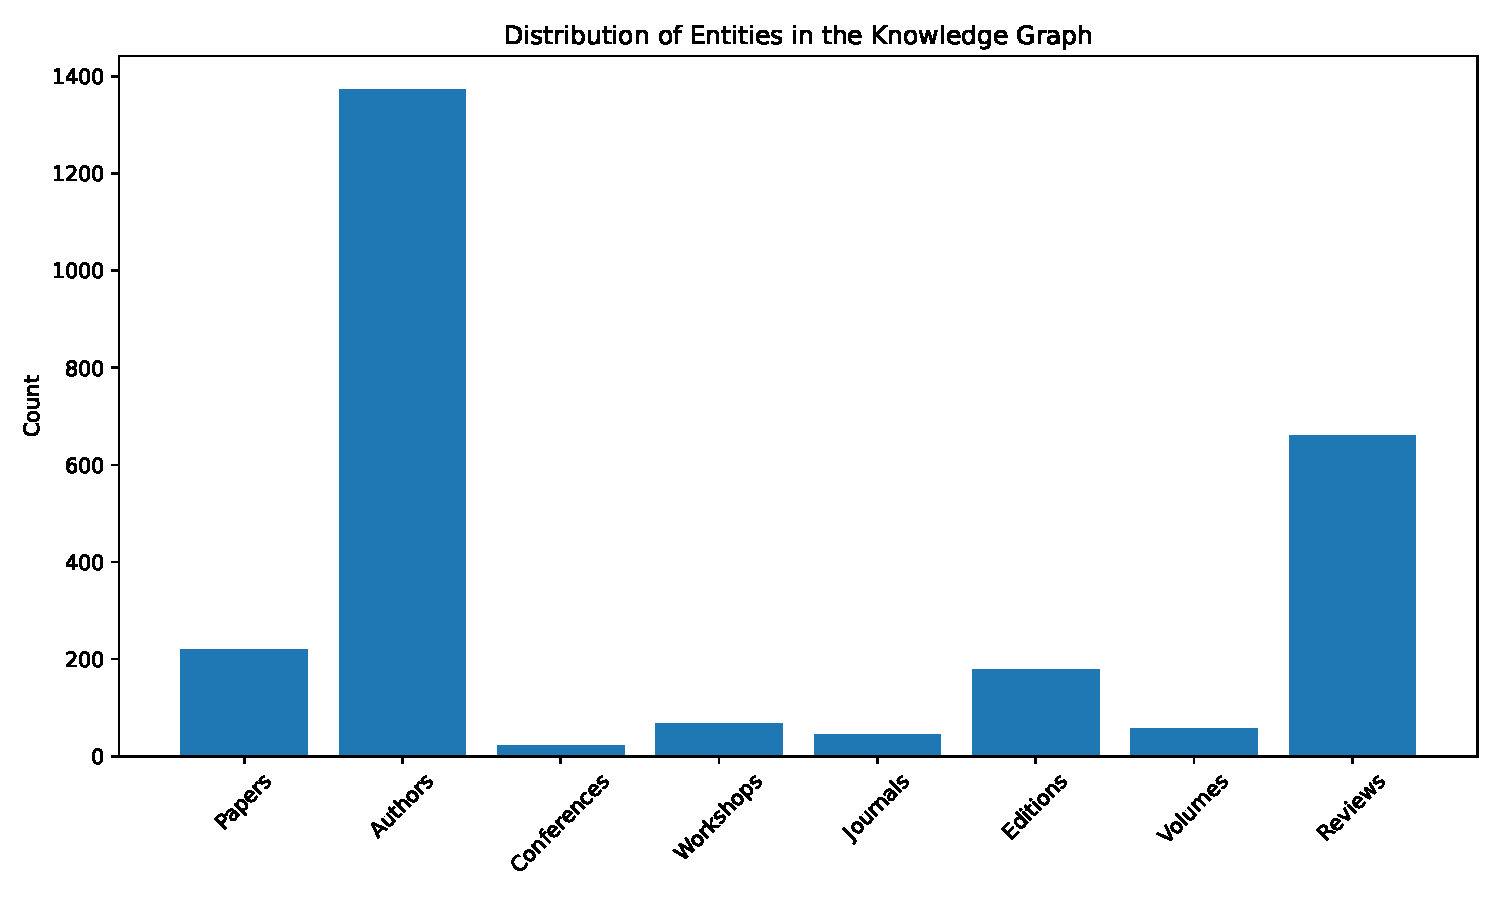
\includegraphics[width=\textwidth]{img/entity_distribution.pdf}
    \caption{Distribution of entities in the knowledge graph. The plot shows the count of each entity type, providing insight into the scale and composition of the knowledge graph.}
    \label{fig:entity_dist}
\end{figure}

The relationships between entities are shown in Figure \ref{fig:relationship_dist}, which illustrates the frequency of different types of connections in the knowledge graph. This helps us understand the density and nature of the relationships in our graph.

\begin{figure}[H]
    \centering
    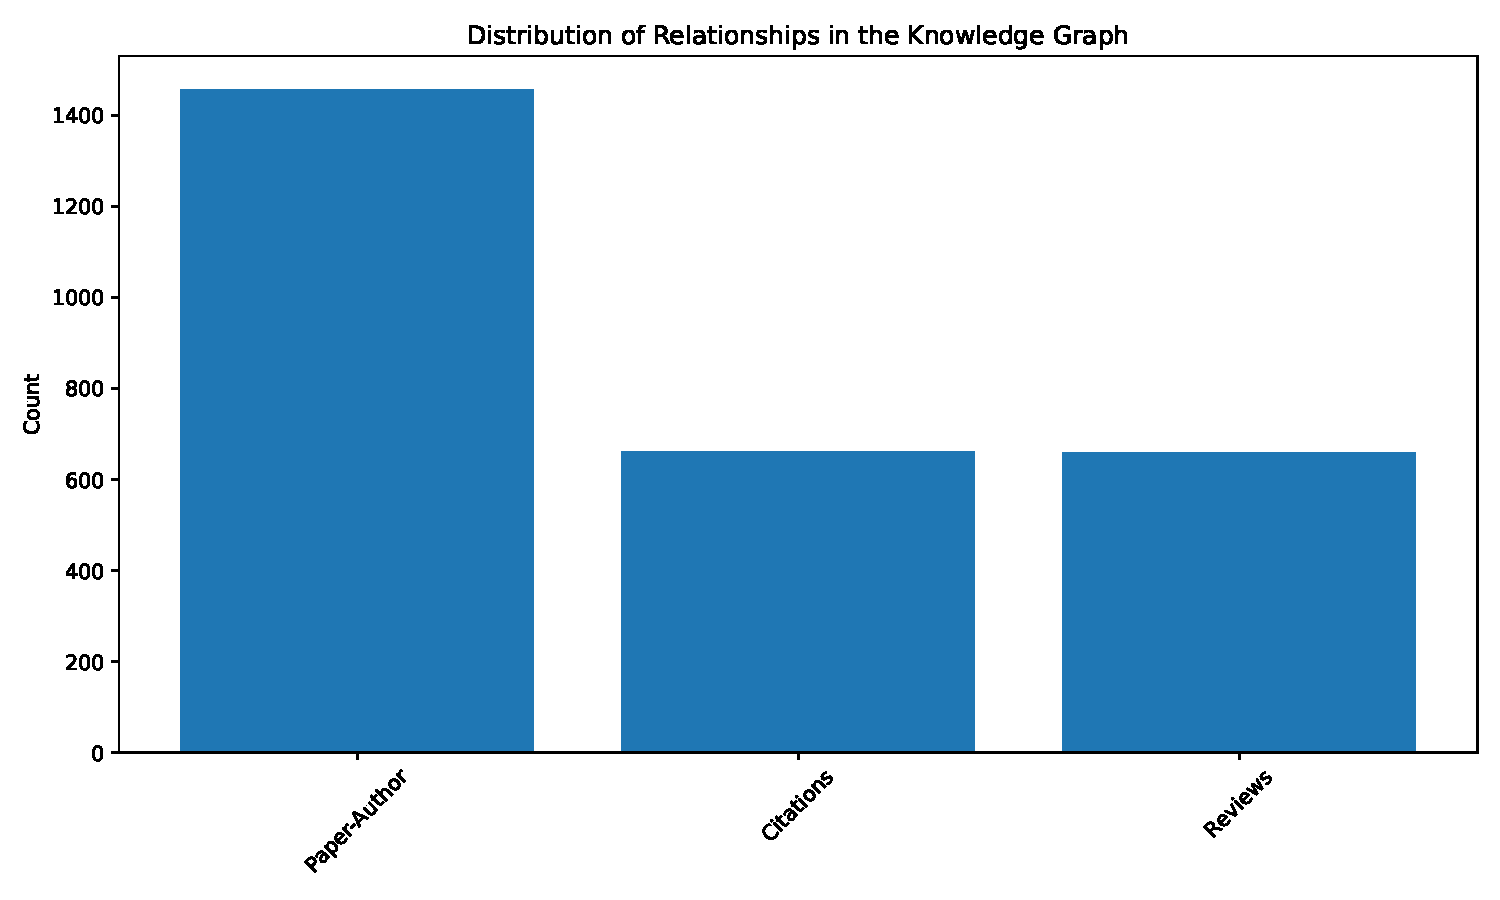
\includegraphics[width=\textwidth]{img/relationship_distribution.pdf}
    \caption{Distribution of relationships in the knowledge graph. The plot shows the count of different types of relationships, highlighting the most common connections between entities.}
    \label{fig:relationship_dist}
\end{figure}

The distribution of publication venues is shown in Figure \ref{fig:venue_dist}, which provides insight into the balance between different types of publication outlets in our dataset.

\begin{figure}[H]
    \centering
    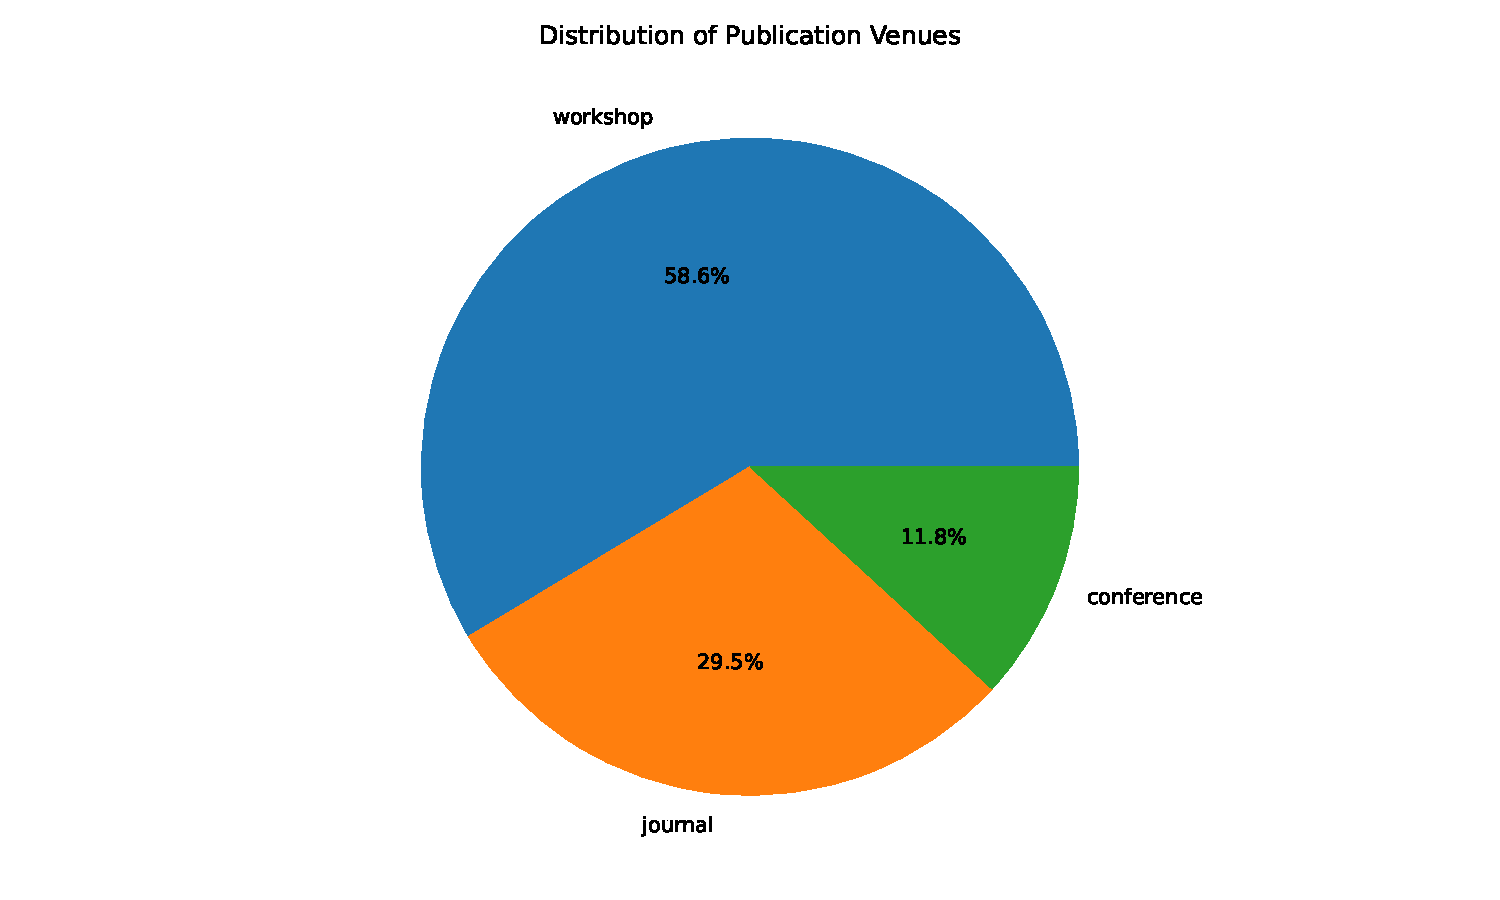
\includegraphics[width=\textwidth]{img/venue_distribution.pdf}
    \caption{Distribution of publication venues. The pie chart shows the proportion of papers published in different types of venues (conferences, workshops, and journals).}
    \label{fig:venue_dist}
\end{figure}

The temporal distribution of papers is shown in Figure \ref{fig:year_dist}, which helps us understand the time span covered by our knowledge graph and any trends in publication frequency.

\begin{figure}[H]
    \centering
    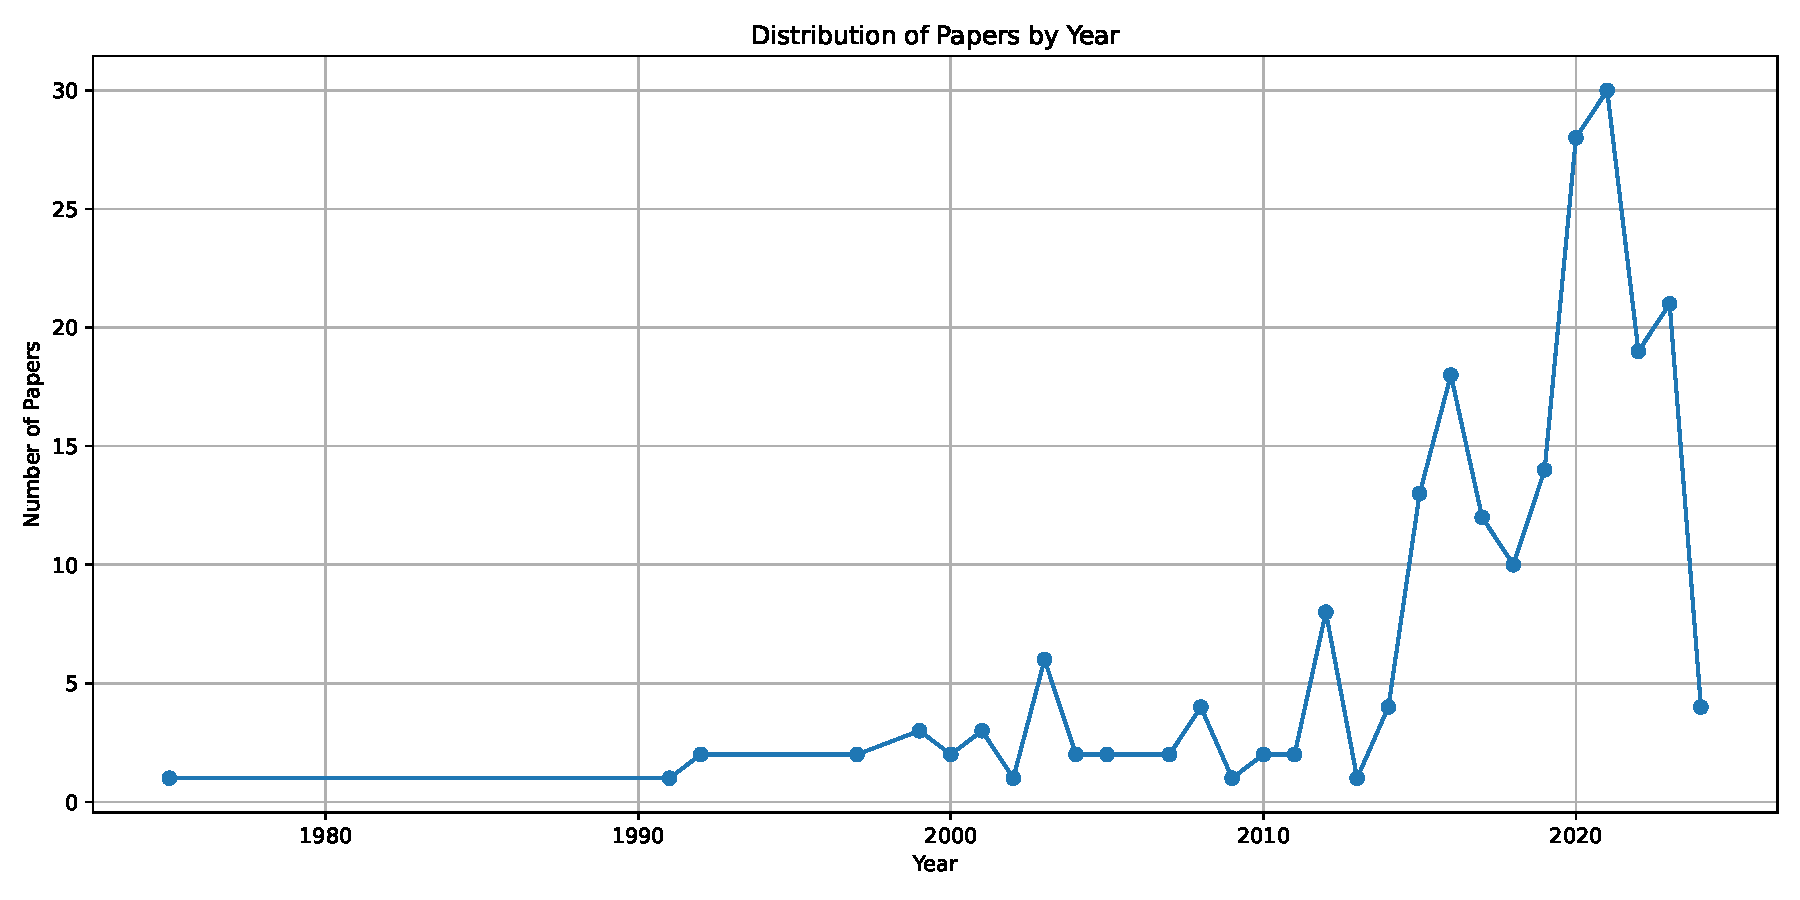
\includegraphics[width=\textwidth]{img/year_distribution.pdf}
    \caption{Distribution of papers by year. The line plot shows the number of papers published each year, revealing trends in publication frequency over time.}
    \label{fig:year_dist}
\end{figure}

Finally, Figure \ref{fig:keyword_dist} shows the most common keywords in the papers, providing insight into the main research topics covered in our knowledge graph.

\begin{figure}[H]
    \centering
    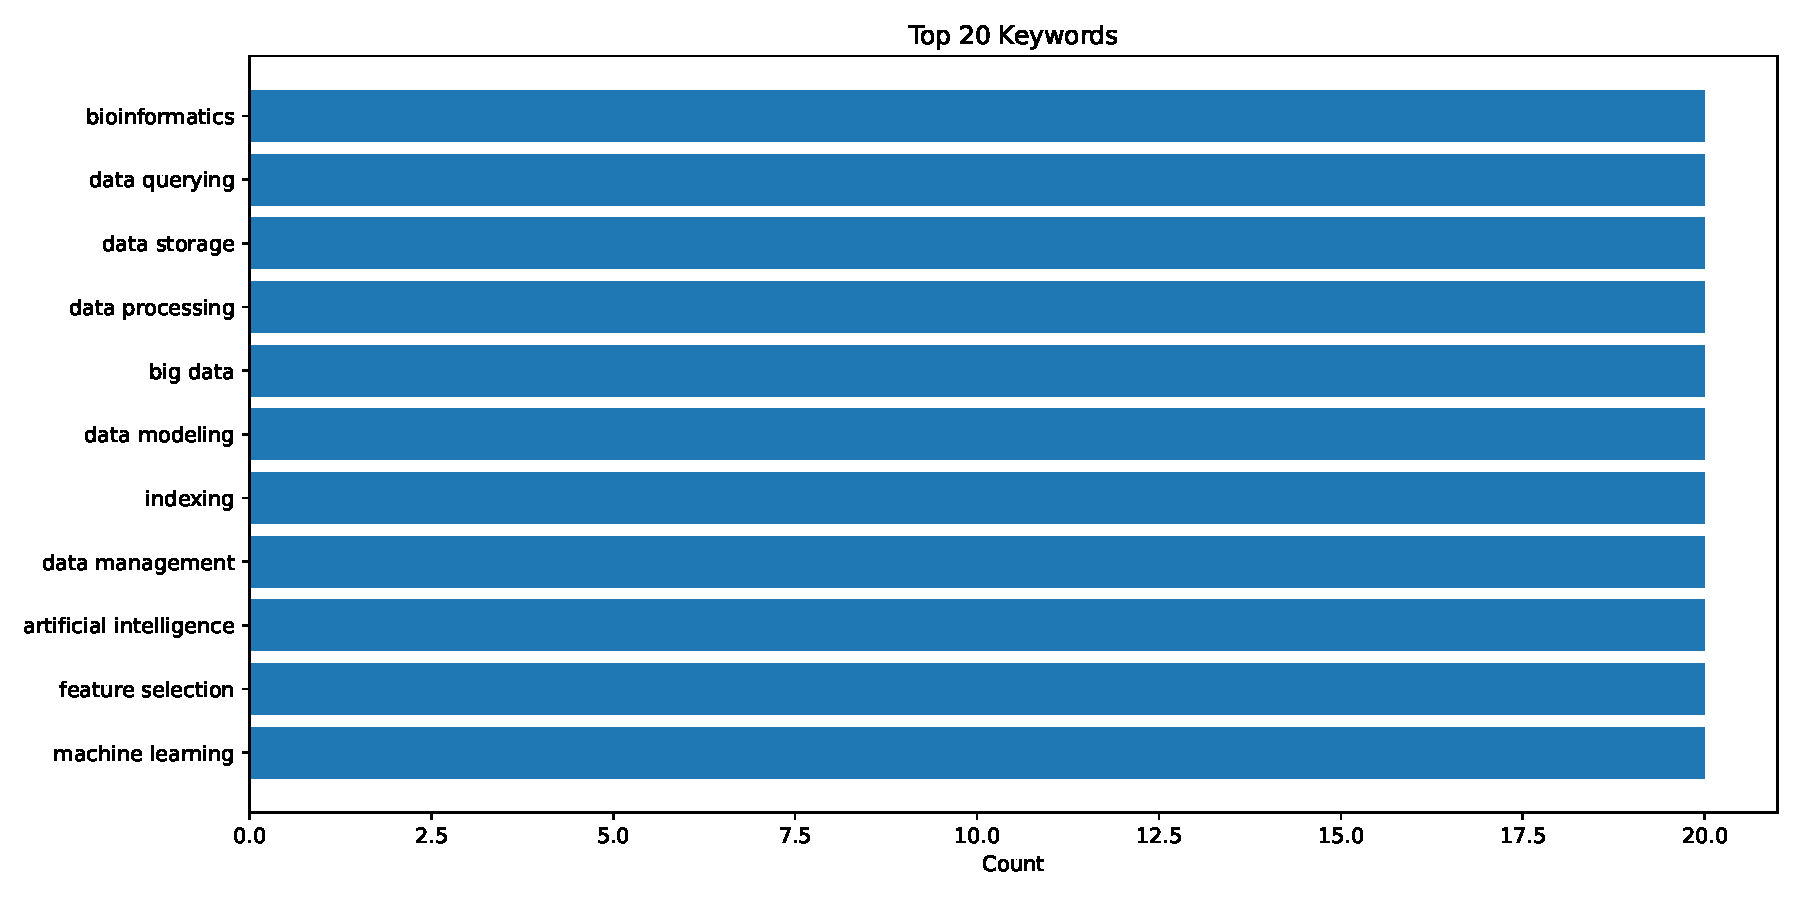
\includegraphics[width=\textwidth]{img/keyword_distribution.pdf}
    \caption{Top 20 keywords in the papers. The horizontal bar chart shows the most frequently occurring keywords, indicating the main research topics in the knowledge graph.}
    \label{fig:keyword_dist}
\end{figure}

These statistics provide valuable insights into the structure and content of our knowledge graph, helping us understand its scale, composition, and the relationships between different entities.

\subsection{Assumptions and Design Decisions}

The implementation makes several key assumptions and design decisions to handle the complexity of the academic publication domain. First, we assume that each paper can be published in exactly one venue (either a conference/workshop edition or a journal volume). This assumption simplifies the relationship structure while maintaining the semantic accuracy of the knowledge graph.

For topics, we assume that keywords are case-sensitive and that whitespace should be preserved. This decision allows for more precise topic matching and querying. The implementation also assumes that keywords are comma-separated in the input data, with each keyword potentially containing internal spaces.

The implementation assumes that author IDs are unique across the entire dataset, allowing for consistent author identification even when the same author appears in multiple papers. This assumption is crucial for maintaining the integrity of author-related relationships.

For temporal data, we assume that years are represented as integers and are valid calendar years. This assumption allows for proper typing of temporal data in the knowledge graph and enables temporal reasoning.

The implementation assumes that each review is uniquely identified by the combination of paper ID and reviewer ID. This assumption allows for proper handling of multiple reviews for the same paper by different reviewers.

Finally, the implementation assumes that the CSV files are properly formatted and that the data types of each column are consistent with their expected usage in the knowledge graph. This includes proper handling of numeric IDs, string values for names and titles, and boolean values for flags like corresponding author status.

These assumptions and design decisions, combined with the robust data validation, ensure that the resulting knowledge graph is both semantically accurate and practically useful for querying and analysis.

\subsection{Querying the Ontology}

To demonstrate the benefits of having an explicit TBOX defined and enabling reasoning, we have created two SPARQL queries that showcase different aspects of our knowledge graph:

\subsubsection{Author's Publication History with Venue Details}
This query demonstrates how we can traverse multiple relationships to get comprehensive information about an author's publications:

\begin{verbatim}
PREFIX rdf: <http://www.w3.org/1999/02/22-rdf-syntax-ns#>
PREFIX rdfs: <http://www.w3.org/2000/01/rdf-schema#>
PREFIX pub: <http://example.org/publication/>
SELECT DISTINCT ?paper ?author ?conference ?venue WHERE{
    ?paper pub:hasAuthor ?author .
    ?author pub:hasName "E. Stefanakis" .
    ?paper pub:isPublishedIn ?proceeding .
    ?edition pub:hasProceedings ?proceeding;
             pub:hasVenue ?venue .
    ?conference pub:hasEdition ?edition .
}
\end{verbatim}

This query showcases several benefits of our TBOX design:
\begin{itemize}
    \item It leverages the explicit relationship between papers and proceedings through \texttt{isPublishedIn}
    \item It uses the connection between editions and their proceedings through \texttt{hasProceedings}
    \item It demonstrates how we can trace a paper's publication path from author to venue through the conference hierarchy
\end{itemize}

\subsubsection{Top Cited Authors}
This query demonstrates how we can perform complex aggregations and rankings using the knowledge graph:

\begin{verbatim}
PREFIX pub: <http://example.org/publication/>
PREFIX rdfs: <http://www.w3.org/2000/01/rdf-schema#>
SELECT ?authorName (COUNT(DISTINCT ?citingPaper) AS ?numCitations)
WHERE {
  ?citingPaper a pub:Paper ;
               pub:cites ?citedPaper .
  ?citedPaper pub:hasAuthor ?author .
  ?author pub:hasName ?authorName .
}
GROUP BY ?authorName
ORDER BY DESC(?numCitations)
LIMIT 10
\end{verbatim}

This query showcases several benefits of our TBOX design:
\begin{itemize}
    \item It uses the \texttt{cites} relationship to track paper citations
    \item It leverages the \texttt{hasAuthor} relationship to connect papers with their authors
    \item It demonstrates how we can perform complex aggregations (counting citations) and rankings (top 10 authors)
    \item The use of \texttt{DISTINCT} ensures we don't count multiple citations of the same paper
\end{itemize}

These queries demonstrate how our TBOX design enables:
\begin{itemize}
    \item Complex relationship traversal across multiple entities
    \item Aggregation and ranking operations
    \item Efficient querying of hierarchical relationships
    \item Clear separation between different types of entities (papers, authors, venues, etc.)
\end{itemize}

\section{Knowledge Graph Embeddings}

\subsection{Importing the Data}

For the creation of Knowledge Graph Embeddings, we carefully selected a subset of the triples from our knowledge graph that capture the most important structural and semantic relationships. The selected data focuses on the core entities and their relationships, which are essential for learning meaningful embeddings.

The selected triples include the following key relationships:

\begin{itemize}
    \item \textbf{Publication Relationships}:
    \begin{itemize}
        \item Papers to Proceedings/Volumes through \texttt{isPublishedIn}
        \item Papers to Authors through \texttt{hasAuthor}
        \item Papers to Corresponding Authors through \texttt{hasCorrespondingAuthor}
        \item Papers to Topics through \texttt{hasKeyword}
    \end{itemize}
    
    \item \textbf{Citation Network}:
    \begin{itemize}
        \item Papers to Papers through \texttt{cites}, capturing the citation network
    \end{itemize}
    
    \item \textbf{Event Structure}:
    \begin{itemize}
        \item Conferences/Workshops to Editions through \texttt{hasEdition}
        \item Editions to Proceedings through \texttt{hasProceedings}
        \item Editions to Venues through \texttt{hasVenue}
    \end{itemize}
    
    \item \textbf{Journal Structure}:
    \begin{itemize}
        \item Journals to Volumes through \texttt{hasVolume}
    \end{itemize}
    
    \item \textbf{Review Process}:
    \begin{itemize}
        \item Papers to Reviews through \texttt{hasReview}
        \item Reviews to Reviewers through \texttt{isAssignedBy}
    \end{itemize}
\end{itemize}

This selection was made with the following considerations:
\begin{itemize}
    \item Focus on structural relationships that define the core topology of the knowledge graph
    \item Inclusion of both hierarchical (e.g., Conference-Edition-Proceedings) and network (e.g., citations) relationships
    \item Coverage of all major entity types (Papers, Authors, Venues, Topics, etc.)
    \item Exclusion of detailed attributes (like review text or paper abstracts) that would not benefit from embedding
\end{itemize}

The selected triples are stored in two TSV files:
\begin{itemize}
    \item \texttt{triples\_kge.tsv}: Contains the triples used for training the KGE models
    \item \texttt{triples\_exploitation.tsv}: Contains additional triples that can be used for downstream tasks
\end{itemize}

This data selection provides a rich foundation for learning embeddings that can capture:
\begin{itemize}
    \item The hierarchical structure of academic publications
    \item The citation network between papers
    \item The relationships between authors and their publications
    \item The topical connections between papers
\end{itemize}

\subsection{Getting familiar with KGEs}

\subsubsection{The most basic model}

For this task, we used the paper with ID \texttt{Paper7e1f6e63f4b06efc18d9d44e46005f79} as our example. We trained a TransE model using PyKEEN with the following configuration:
\begin{itemize}
    \item Embedding dimension: 50
    \item Number of epochs: 20
    \item Learning rate: 0.01
    \item Training/validation/test split: 80/10/10 (stratified by relation type)
    \item Negative sampling: 1 negative sample per positive triple
    \item Loss function: Margin ranking loss with margin of 1.0
\end{itemize}

The model was trained on GPU (CUDA) to accelerate the learning process. The training data was loaded from \texttt{triples\_kge.tsv} and automatically split by PyKEEN to ensure a balanced distribution of relation types across the splits.

To find the most likely cited paper according to TransE:
\begin{enumerate}
    \item Get the paper's embedding vector $h$
    \item Get the citation relation's embedding vector $r$
    \item Calculate expected cited paper embedding as $h + r$
\end{enumerate}

To find the most likely author of a paper:
\begin{enumerate}
    \item Get the paper's embedding vector $h$
    \item Get the author relation's embedding vector $r$
    \item Calculate expected author embedding as $h - r$
\end{enumerate}

We implemented these calculations in Python using PyKEEN and PyTorch. The code finds the closest entity to the expected embedding vector using Euclidean distance. For our example paper, the model predicted:
\begin{itemize}
    \item Most likely cited paper: \texttt{Paperd114e1de831cc6bc29233d024f137d48}
    \item Most likely author: \texttt{Author67936dfd5e69470e080a42e83032e605}
\end{itemize}

It is worth noting that the predicted paper and author are correct types only because we added explicit type filtering to the model. If we did not add this filtering, the model would have predicted a Review and an Author, respectively, which are incorrect types. However, these entity type constraints are substantiated by previous literature: [TODO: add references, "Improving Knowledge Graph Embeddings with Inferred Entity Types"]

\subsubsection{Improving TransE}

The TransE model, while simple and interpretable, has significant limitations when dealing with complex relationships. Let's analyze these limitations and explore potential solutions.

\paragraph{One-to-Many/Many-to-One Relationships}
Consider a knowledge graph with the following triples:
\begin{itemize}
    \item (Author1, writes, Paper1)
    \item (Author2, writes, Paper1)
    \item (Author1, writes, Paper2)
\end{itemize}

In TransE, the model tries to satisfy $h + r \approx t$ for each triple. For the first two triples, this means:
\begin{align*}
    \text{Author1} + \text{writes} \approx \text{Paper1} \\
    \text{Author2} + \text{writes} \approx \text{Paper1}
\end{align*}

This leads to $\text{Author1} \approx \text{Author2}$, which is incorrect since they are different authors. Similarly, for the first and third triples:
\begin{align*}
    \text{Author1} + \text{writes} \approx \text{Paper1} \\
    \text{Author1} + \text{writes} \approx \text{Paper2}
\end{align*}

This forces $\text{Paper1} \approx \text{Paper2}$, which is also incorrect. These contradictions demonstrate TransE's inability to properly model one-to-many and many-to-one relationships.

\paragraph{Solving One-to-Many Issues}
TransH was specifically designed to address this limitation. Instead of translating entities in the same space, TransH projects entities onto relation-specific hyperplanes. This allows the same entity to have different projections for different relationships, effectively solving the contradiction we saw with TransE. For example, Author1 and Author2 can have different projections on the "writes" hyperplane while maintaining their distinct identities in the original space.

\paragraph{Symmetric Relationships}
Consider a symmetric relationship like "collaboratesWith" between authors. In TransE, for the triples:
\begin{itemize}
    \item (Author1, collaboratesWith, Author2)
    \item (Author2, collaboratesWith, Author1)
\end{itemize}

The model would try to satisfy:
\begin{align*}
    \text{Author1} + \text{collaboratesWith} \approx \text{Author2} \\
    \text{Author2} + \text{collaboratesWith} \approx \text{Author1}
\end{align*}

This would require $\text{collaboratesWith} \approx \text{Author2} - \text{Author1}$ and $\text{collaboratesWith} \approx \text{Author1} - \text{Author2}$, which can only be satisfied if $\text{collaboratesWith} \approx \vec{0}$ (the zero vector). This is a degenerate solution that doesn't capture the true meaning of the relationship. The scores for both triples should indeed be the same since collaboration is symmetric, but TransE cannot properly model this symmetry without resorting to this trivial solution.

\begin{figure}[H]
    \centering
    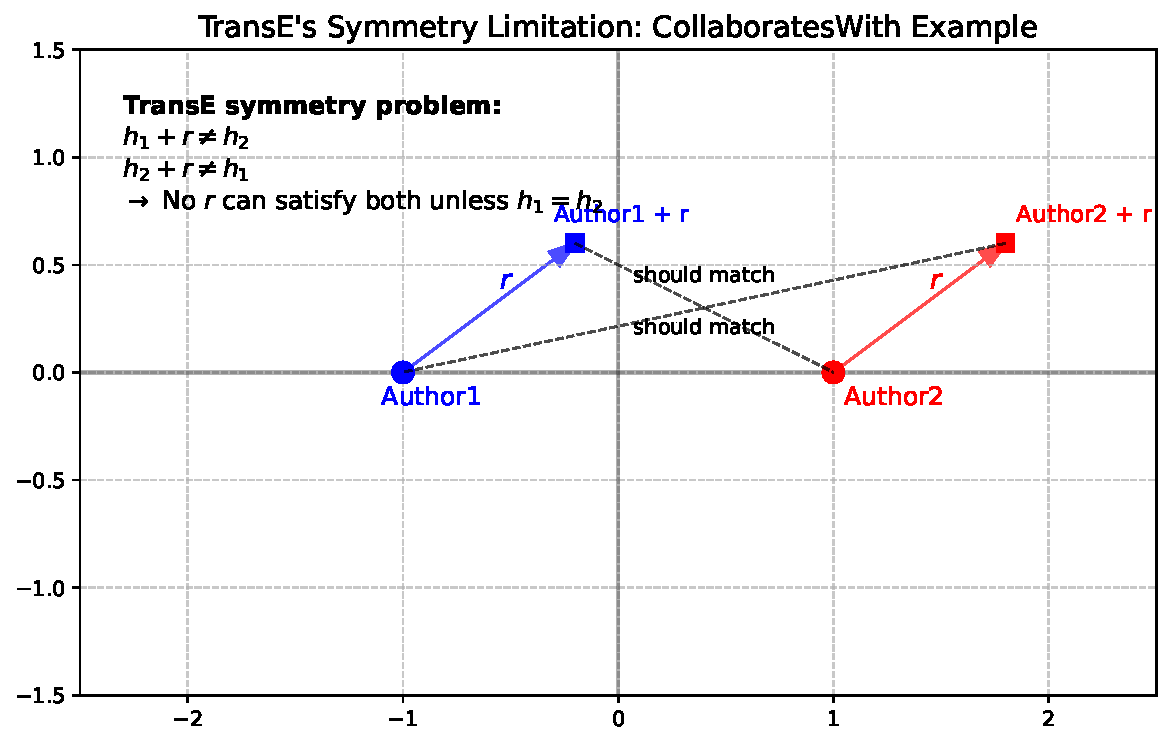
\includegraphics[width=0.8\textwidth]{img/transe_symmetry.pdf}
    \caption{Visualization of TransE's symmetry problem. The arrows show how TransE tries to model the symmetric "collaboratesWith" relationship between two authors. For the relationship to be symmetric, the relation vector would need to be the zero vector, which is a degenerate solution that doesn't capture the true meaning of collaboration.}
    \label{fig:transe_symmetry}
\end{figure}

As shown in Figure \ref{fig:transe_symmetry}, when trying to model a symmetric relationship like "collaboratesWith" between two authors, TransE faces a fundamental problem. The model needs to find a relation vector that, when added to Author1, points to Author2, and when added to Author2, points to Author1. This is only possible if the relation vector is the zero vector, which is a degenerate solution that doesn't capture any meaningful information about the relationship. This is why TransE struggles with symmetric relationships unless it resorts to this trivial solution.

\paragraph{RotatE's Solution to Symmetry}
RotatE solves the symmetry problem by using complex numbers and rotation in the complex plane. Instead of adding vectors like TransE, RotatE multiplies complex numbers, where each entity and relation is represented as a complex number. For a symmetric relationship, RotatE can achieve symmetry by using a rotation of 180 degrees ($\pi$ radians).

\begin{figure}[H]
    \centering
    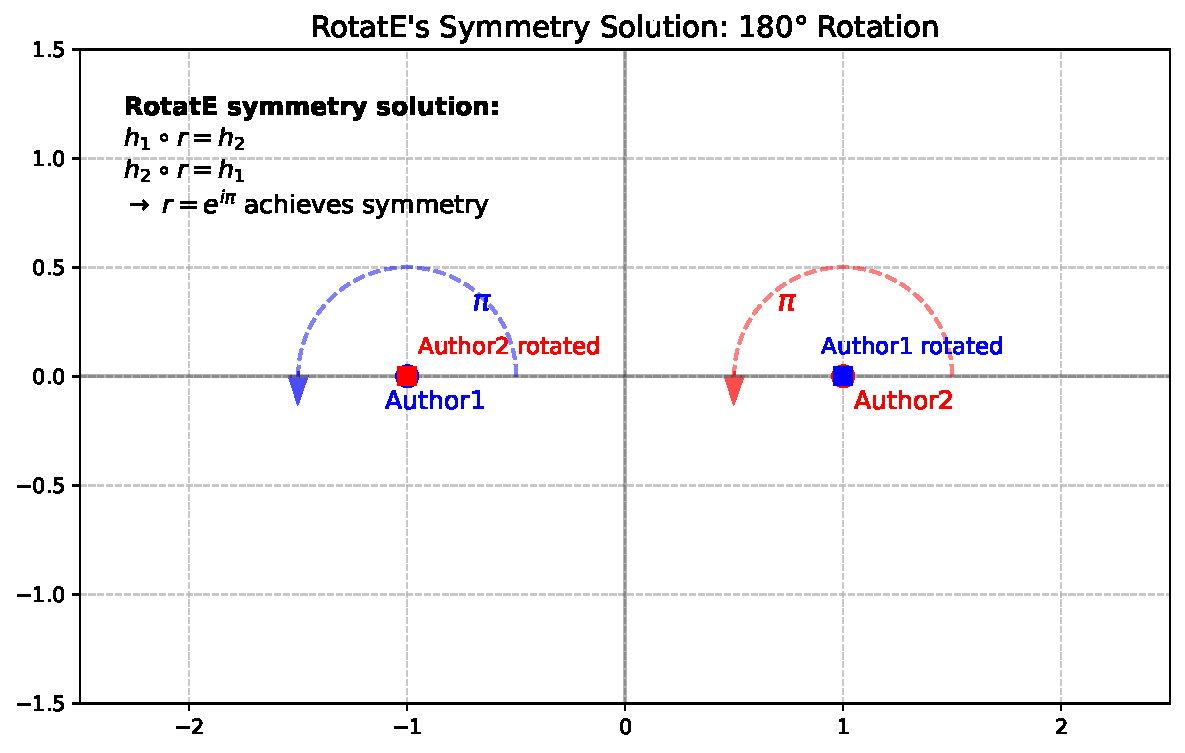
\includegraphics[width=0.8\textwidth]{img/rotate_symmetry.pdf}
    \caption{Visualization of how RotatE handles symmetric relationships. The dashed arcs show the 180-degree rotations that transform Author1 to Author2 and vice versa. The relation $r = e^{i\pi}$ (rotation by $\pi$ radians) achieves perfect symmetry.}
    \label{fig:rotate_symmetry}
\end{figure}

As shown in Figure \ref{fig:rotate_symmetry}, RotatE can model symmetric relationships by using a rotation of $\pi$ radians. When we rotate Author1 by $\pi$ radians, we get Author2, and when we rotate Author2 by $\pi$ radians, we get Author1. This is achieved by setting the relation vector $r = e^{i\pi}$, which represents a 180-degree rotation. This solution is not degenerate and properly captures the symmetric nature of the relationship.

\paragraph{DistMult's Natural Symmetry}
DistMult is another model that naturally handles symmetric relationships without requiring any special considerations. Unlike TransE and RotatE, which use vector addition and rotation respectively, DistMult uses a simple element-wise multiplication (Hadamard product) between entity and relation vectors. The scoring function for a triple $(h, r, t)$ is:

\begin{align*}
    f(h, r, t) = \sum_{i=1}^d h_i \cdot r_i \cdot t_i
\end{align*}

where $h_i$, $r_i$, and $t_i$ are the $i$-th components of the head entity, relation, and tail entity vectors respectively. This formulation naturally handles symmetric relationships because the scoring function is symmetric with respect to the head and tail entities when the relation vector has symmetric components. For example, if we have a symmetric relationship like "collaboratesWith", the relation vector will have components that are symmetric around zero, making the score the same regardless of the order of the entities.

This property makes DistMult particularly well-suited for modeling symmetric relationships in knowledge graphs, as it doesn't require any special handling or constraints to achieve symmetry. However, this same property can be a limitation when modeling asymmetric relationships, as the model cannot distinguish between different directions of the same relation.

\subsection{Training KGEs}

We implemented and evaluated five different Knowledge Graph Embedding (KGE) models: TransE, TransH, RotatE, DistMult, and ComplEx. The training pipeline was implemented in Python using the PyKEEN library, with support for inverse triples, cross-validation, and hyperparameter optimization.

\subsubsection{Training Pipeline}

The training process follows these steps:

\begin{enumerate}
    \item \textbf{Data Preparation}: The RDF triples were preprocessed into subject-predicate-object format and used to create labeled triples for the embedding models. The dataset was split using 3-fold cross-validation to ensure a more robust performance estimate.
    
    \item \textbf{Hyperparameter Optimization}: For each model, we performed a grid search over the following hyperparameters:
    \begin{itemize}
        \item Embedding dimension: [50, 100, 200]
        \item Number of negative samples per positive triple: [1, 3, 5]
        \item Learning rate: [0.001, 0.0005, 0.0001]
        \item Batch size: [64, 128, 256]
    \end{itemize}
    
    \item \textbf{Model Training}: Models were trained using the Adam optimizer, with early stopping enabled (patience = 5, relative\_delta = 0.002) to prevent overfitting. All experiments were conducted using CPU due to hardware constraints.

    \item \textbf{Evaluation}: Each trained model was evaluated on the test fold using the following ranking-based metrics:
    \begin{itemize}
        \item Mean Reciprocal Rank (MRR)
        \item Hits@1: Proportion of true triples ranked first
        \item Hits@3: Proportion of true triples in the top 3 predictions
        \item Hits@10: Proportion of true triples in the top 10 predictions
    \end{itemize}
\end{enumerate}

\subsubsection{Results and Interpretation}

\begin{table}[H]
    \centering
    \input{tab/model_comparison.csv}
    \caption{Performance comparison of KGE models on our knowledge graph. Higher values indicate better ranking performance.}
    \label{tab:model_comparison}
\end{table}

The best-performing model was \textbf{TransH}, which achieved an MRR of 0.151 and Hits@10 of 0.207. This result highlights TransH’s ability to better model diverse and complex relation types by introducing a relation-specific hyperplane for entity projections. The inclusion of inverse triples also significantly improved the performance of all models by doubling the observed relation directions.

\textbf{DistMult} performed similarly well, particularly in Hits@1 (11.6\%), despite its known limitation in handling asymmetric relations. This suggests that a substantial portion of the graph may involve symmetric or quasi-symmetric predicates, such as \texttt{hasKeyword} or \texttt{hasReview}.

\textbf{RotatE} showed moderate performance, indicating some ability to capture more complex relational patterns such as symmetry and inversion. However, it was outperformed by simpler bilinear and projection-based models, possibly due to underfitting or suboptimal hyperparameters in this setting.

\textbf{TransE}, as expected, yielded the lowest results (MRR: 0.025), as its simplistic translational model struggles with multi-relational structures and many-to-many relations, which are common in academic metadata (e.g., multiple authors per paper).

\textbf{ComplEx} was tested with and without inverse triples, but even with inverses, it failed to outperform other models. This could be attributed to several factors: its sensitivity to initialization, potential mismatch between model capacity and the dataset size (relatively small at $\sim$4600 triples), or insufficient tuning of regularization parameters.

\paragraph{Why are the scores low?}
Overall, absolute performance scores across all models were modest. This is likely due to the limited size and sparsity of the knowledge graph (4636 triples across 2943 entities and 12 relations), which restricts the models’ ability to generalize. Additionally, the skewed distribution of relations—where some are highly frequent (e.g., \texttt{hasAuthor}) and others sparse—makes learning consistent embeddings challenging. The lack of type constraints or schema-level information may also contribute to the difficulty of distinguishing between semantically plausible and implausible triples.

\subsection{Exploitation analysis}

To explore the temporal dynamics of author behavior in the research graph, we applied clustering over the learned entity embeddings of authors, split by year. Specifically, we trained a KMeans model with $k=5$ on the subset of author embeddings corresponding to each year from 2015 to 2023. This allowed us to observe how clusters of semantically similar authors (based on their roles and relations in the graph) evolve over time.

Figure~\ref{fig:cluster_evolution} shows the size of each cluster across the analyzed years. Several insights emerge from this visualization:

\begin{itemize}
    \item \textbf{Cluster Volatility:} Certain clusters, such as Cluster 1, show sharp fluctuations — peaking dramatically in 2019, then collapsing the following year. This could be tied to a high-impact event or conference held that year which attracted a temporary spike in activity from a subset of authors.
    
    \item \textbf{Stability and Growth:} Clusters like Cluster 0 and Cluster 4 demonstrate more stable growth trends, suggesting that they represent core, persistently active author groups.

    \item \textbf{Rotational Membership:} The sizes of Clusters 2 and 3 fluctuate in a pattern suggesting that authors may be rotating between them over the years. This may reflect shifts in topical focus or institutional affiliation.

    \item \textbf{Cluster Interpretation:} Given that embeddings encode structural information (e.g., coauthorship, venues, and citations), we hypothesize that clusters are driven by a combination of shared publication venues, coauthor networks, and thematic areas. Further inspection of cluster members supports this, showing that certain clusters are enriched for authors publishing in specific conferences or topics.
\end{itemize}

This analysis reveals that embedding-based clustering can capture real structural patterns and shifts in academic activity, opening the door to trend analysis, author recommendation, and community detection in scholarly knowledge graphs.

\begin{figure}[H]
    \centering
    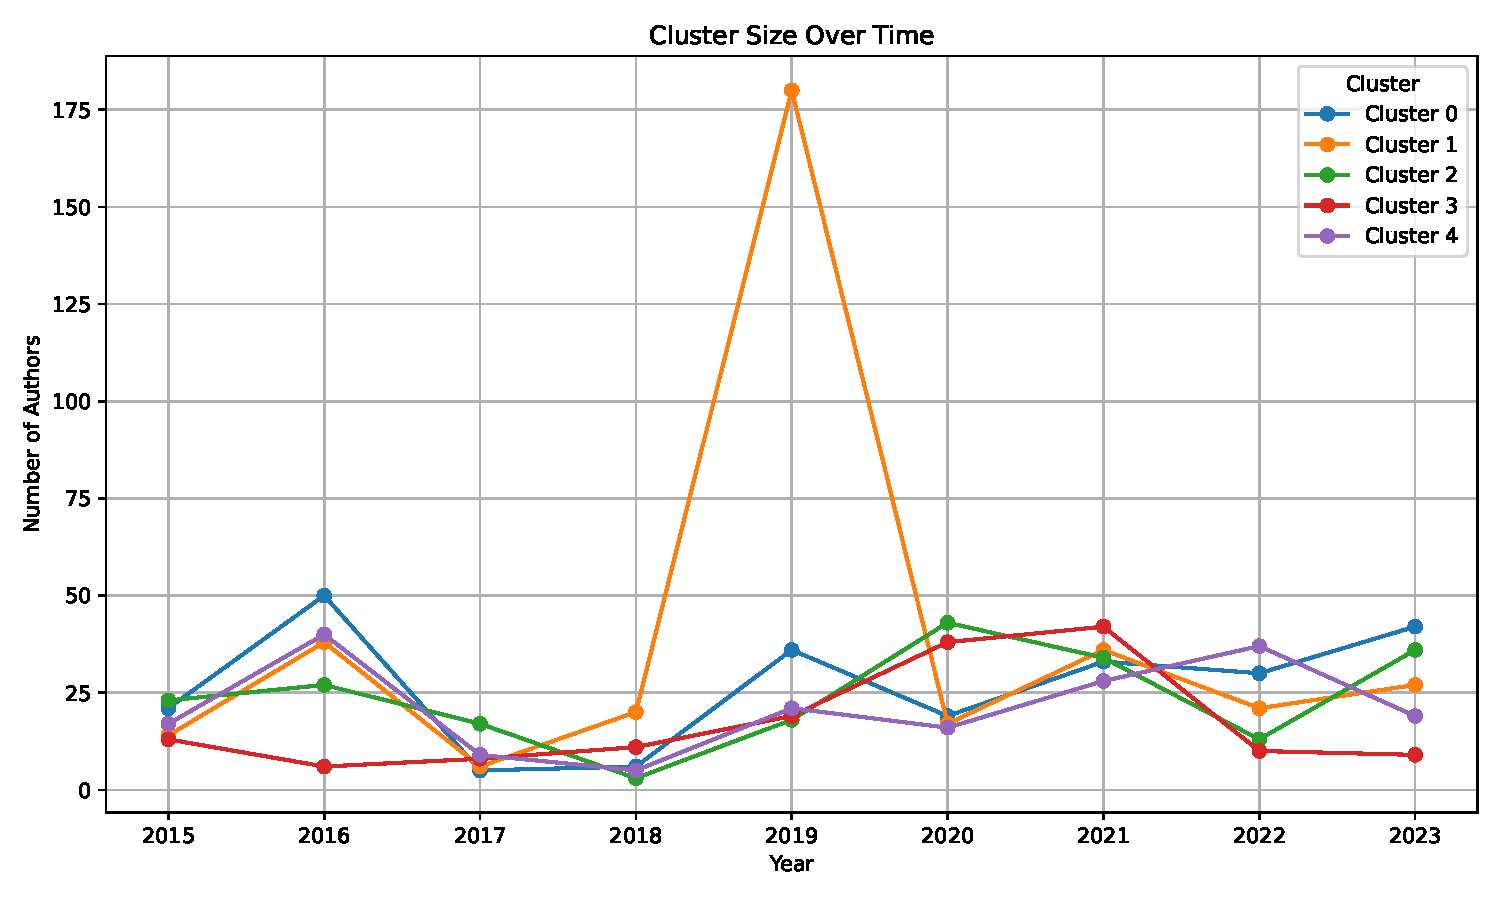
\includegraphics[width=0.95\textwidth]{img/cluster_distribution_over_time.pdf}
    \caption{Author cluster size over time. Each line represents one cluster (from KMeans with $k=5$), and the vertical axis shows the number of authors in that cluster in a given year.}
    \label{fig:cluster_evolution}
\end{figure}

\subsection{Keyword Analysis by Cluster}

To further interpret the semantic coherence of the discovered author clusters, we extracted the most frequent keywords used by each cluster in each year. For this, we associated authors with their published papers, collected the \texttt{keywords} field from those papers, and aggregated them per cluster and year. The top terms per cluster were then counted to identify dominant research themes.

Table~\ref{tab:cluster_keywords} summarizes a subset of this analysis. The complete results are available in the supplementary CSV file (\texttt{doc/cluster\_keywords\_by\_year.csv}).

\begin{table}[H]
\centering
\scriptsize
\pgfplotstabletypeset[
    col sep=comma,
    string type,
    columns/year/.style={column name=Year, column type={c}},
    columns/cluster_id/.style={column name=Cluster, column type={c}},
    columns/keyword/.style={column name=Keyword, column type={c}},
    columns/count/.style={column name=Count, column type={c}},
    every head row/.style={
        before row=\toprule, after row=\midrule
    },
    every last row/.style={after row=\bottomrule}
]{doc/cluster_keywords_2022.csv}
\caption{Top keywords per cluster and year extracted from author clusters over time.}
\label{tab:cluster_keywords_csv}
\end{table}

\paragraph{Observations:}

\begin{itemize}
    \item \textbf{Persistent Topics:} Clusters focused on \textit{data processing}, \textit{data storage}, and \textit{machine learning} appear repeatedly across multiple years, indicating sustained research interest.
    
    \item \textbf{Emerging Trends:} \textit{Artificial intelligence} appears as a dominant term only after 2019, reflecting its recent rise in prominence within the community.

    \item \textbf{Shifting Focus:} Cluster 1's transition from \textit{data processing} in 2019 to \textit{artificial intelligence} by 2023 may suggest topic drift among a subset of authors.

    \item \textbf{Specialized Clusters:} Cluster 2 consistently shows strong signals for \textit{bioinformatics}, implying a domain-specific author group.

    \item \textbf{Consolidation:} In 2022, both \textit{big data} and \textit{data storage} peaked together in Cluster 0, suggesting a convergence of themes under a unified group.
\end{itemize}

This temporal keyword distribution complements the clustering results, confirming that clusters are not only structurally coherent (via embeddings), but also semantically meaningful and traceable over time.


\end{document} 